\clearpage
\setcounter{page}{1}

\section{Einführung in FEAPpv}


Die kommenden \"Ubungen werden sich mit der Implementierung von Elementen innerhalb der Finite Elemente Software FEAPpv befassen.
FEAPpv ist f\"ur die Nutzung auf Unix"=\slash{}Linux"=Systemen konzipiert, die Software Cygwin erm\"oglicht jedoch auch die Nutzung unter Windows. 
Die Installation innerhalb der Cygwin"=Umgebung ist nachfolgend beschrieben.
%Nach der Installation und einer kurzen Einf\"uhrung
% in das Programm und in Fortran~77
%sollen zwei einfache Materialgesetze implementiert und zur Berechnung einer Membran genutzt werden.


\subsection*{Installation von FEAPpv unter Cygwin}
Zur erstmaligen Installation von FEAPpv im CIP"~Pool m\"ussen folgende Schritte durchgef\"uhrt werden:
\begin{enumerate}[label=\arabic*.)]
 \item ein Cygwin64"=Terminal \"offnen,
 \item Homeverzeichnis von Cygwin unter C:/cygwin64/home/\verb|<|RUB-login\verb|>| \"offnen und am Ende der Datei \verb|.bashrc| die folgenden Zeilen einf\"ugen:\\[2mm]
 \verb|export FEAPPVHOME4_1=/cygdrive/z/feappv41/ver41|\\
 \verb|alias feappv='$FEAPPVHOME4_1/main/feappv.exe'|,\\
 \verb|alias gnuplot="/cygdrive/c/'Program Files'/blueCFD-Core-2017/msys64/|...\\
 ...\verb|mingw64/bin/gnuplot.exe"|,\\[2mm]
 anschlie{\ss}end die Datei zur sp\"ateren Nutzung auf das eigene Laufwerk Z sichern,
 \item den bereitgestellten Ordner \verb|feappv41| im pers\"onlichen Laufwerk Z ablegen,
  \item unter alle Programme/Cygwin-X auf \enquote{XWin Server} klicken und im Anschluss durch Rechtsklick auf das Cygwin"=Symbol in der Taskleiste unter Systemwerkzeuge ein Cygwin"=Terminal starten,
 \item mit dem Befehl \verb|cd /cygdrive/z/feappv41/ver41| in den Ordner \verb|feappv41/ver41| navigieren und das Programm mit dem Befehl \verb|make install| kompilieren,
 \item zum Testen des Programms in den Ordner \verb|calc/0_beispiel| wechseln, den Befehl \verb|feappv| eingeben und den weiteren Anweisungen folgen.
\end{enumerate}

Wenn \"Anderungen am Programm vorgenommen werden, muss dieses neu kompiliert werden.
Das erfolgt durch Eingabe von \verb|make| im Ordner \verb|ver41|.
Einige h\"aufig verwendete Konsolen"=Befehle sind auf der nächsten Seite zusammengefasst.

\clearpage



\subsubsection*{Einige nützliche Konsolenbefehle}

\begin{minipage}{\textwidth}
\begin{tabular}{ll}
 Befehl                        & Auswirkung \\\toprule
 ls                            & Auflisten des Inhalts des aktuellen Verzeichnisses\\
 cd \verb|<|Pfad\verb|>|       & aus dem aktuellen Verzeichnis nach <Pfad> navigieren\\
 cd ..                         & eine Verzeichnisebene nach oben wechseln\\
%  cd \~                       & ins Homeverzeichnis von Cygwin navigieren\\
 cd /cygdrive/z                & ins Laufwerk Z navigieren\\
 clear                         & Konsoleninhalt l\"oschen\\
 exit                          & Konsole schlie{\ss}en\\\midrule
\end{tabular} 
\end{minipage}\medskip




\subsubsection*{Kurzübersicht FEAP-Kommandos}

\begin{tabular}{ll}
\verb/tang,,1/ & start one iteration step\\
\verb/disp,,/{\sl num} & print coordinates and displacements of node {\sl num}\\
\verb/plot/    & enter the plot-command-environment\\
\verb/plot,/\verb/mesh/    & show mesh\\
\verb/plot,/\verb/node,/{\sl num}    & show number of node {\sl num}\\
& {\sl num}=blank, plot all numbers)\\
\verb/plot,/\verb/elem,/{\sl num}    & show number of element {\sl num}\\
& ({\sl num}=blank, plot all numbers)\\
\verb/plot,/\verb/defo,/{\sl factor}\verb/,1/ & switch to deformed configuration with scaling by {\sl factor}\\
\verb/plot,/\verb/unde/    & switch to undeformed configuration\\
\verb/plot,/\verb/boun/    & show boundary conditions\\
\verb/plot,/\verb/load/    & show loads\\
\verb/plot,/\verb/post/    & start/end plot to postscript-file\\
\verb/plot,/\verb/stre,/{\sl index}\verb/,,/{\sl flag} & plot stress distribution,\\
& {\sl index}: 1$\rightarrow\sigma_{11}$, 2$\rightarrow\sigma_{22}$, $\ldots$ ;
{\sl flag}: 0=mesh, 1=no mesh\\
\verb/plot,/\verb/wipe/    & clear plot window
\end{tabular}\medskip

\textit{Hinweis}:
% (\verb/plot,/) kann weggelassen werden, wenn die plot-Befehlsumgebung in einer vorherigen Zeile bereits geöffnet ist.
Weitere Befehle und Erläuterungen lassen sich dem in FEAPpv enthaltenden Benutzerhandbuch unter dem Dateipfad 
\verb| ver41/manual/manual41.pdf  | entnehmen.

\medskip




\subsubsection*{Hinweis zum Erstellen von Plots mithilfe von $\tt gnuplot$}

$\tt Gnuplot$ ist ein skript- bzw. kommandozeilengesteuerte Computerprogramm zur grafischen Darstellung von Daten.
Entsprechende Skriptdateien werden mit folgendem Befehl ausgeführt:

\ebn
\verb| gnuplot <scriptname>.gnu |
\een





\subsection{Cook's Membran Problem}


\begin{minipage}{0.4\textwidth}
Eine FEAPpv-kompatible Input-Datei für das dargestellte Problem soll erstellt werden.
Nutzen sie die in dieser Übung bereitgestellte Beispieldatei $\tt I\_test$ als Vorlage und erzeugen sie die FE-Lösung für die folgenden Netzverfeinerungsstufen:

\begin{center}
\begin{tabular}{rc|c}
 & \multicolumn{2}{c}{Elemente in}\\
 & x-Richtung ($nx$) & y-Richtung ($ny$) \\\cline{2-3}
1) & 10 & 5\\
2) & 20 & 10\\
3) & 40 & 20\\
4) & 80 & 40\\
5) & 160 & 80\\
\end{tabular}
\end{center}
\end{minipage}
%
\hfill
%
\begin{minipage}{0.54\textwidth}
 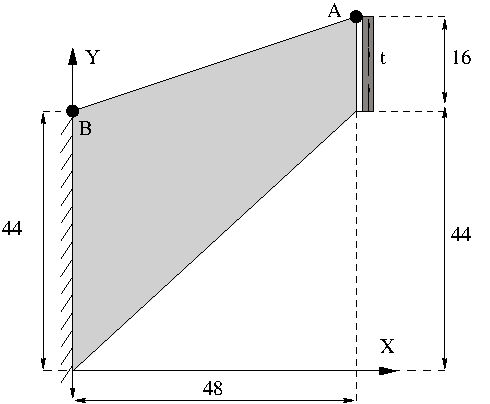
\includegraphics[width=0.9\textwidth]{fig/ue6_cm_problem_description.pdf}
 \captionof{figure}{Cook's Membran Geometrie}\smallskip
Materialparameter:
$E = 210000\,\mbox{MPa} \,,\; \nu = 0.3$

Neumann-Randbedingung:
$t = 5000\,\mbox{MPa}$
\end{minipage}

\enab
  \item Berechnen Sie die Verschiebung in Vertikalrichtung im Punkt $\tt A$ für die verschiedenen Netzverfeinerungsstufen 1)-5) und Veranschaulichen Sie die Ergebnisse in einem ensprechenden Diagramm.

  \textit{Hinweis:} Speichern Sie dazu die jeweiligen Berechnungsergebnisse in der Datei \verb| u-nelem.dat| und nutzen Sie das beigefügte Gnuplot-Skript \verb| u-nelem.gnu|.
 % 
  \item Erzeugen Sie die folgenden Plots
  \begin{itemize}
    \item Netz im Ausgangszustand mit Dirichiet- und Neumann Randbedingungen basierend auf Netzverfeinerungsstufe 2),
    \item Geometrie im Verformten Zustand mit den Spannungs-Contourplots $\sigma_{11}, \sigma_{22}, \sigma_{33}$ basierend auf Netzverfeinerungsstufe 5).
  \end{itemize}
\enae


% \clearpage
% 
% \begin{figure}[h]
% 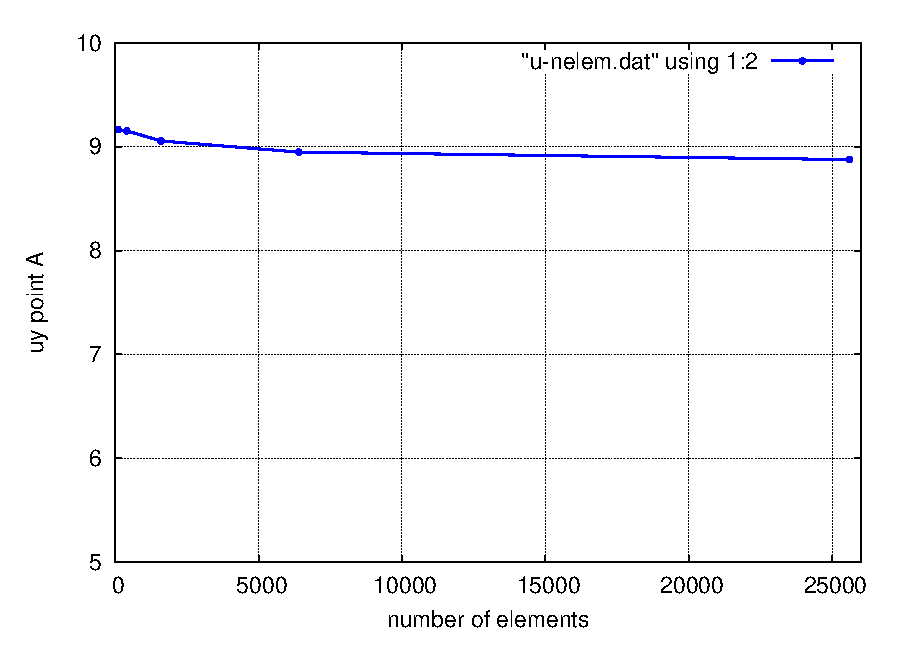
\includegraphics[width=0.9\textwidth]{fig/ue6_u-nelem.eps}
% \caption{Verschiebung im Punkt {\sf A} basierend auf Verfeinerung 1) - 5)}
% \end{figure}
% \begin{figure}[h]
% \includegraphics[width=0.9\textwidth]{mesh_bounds_loads.eps}\\
% \caption{Undeformed mesh (discretization 2) with boundary conditions and applied loads.}
% \end{figure}
% 
% \clearpage
% 
% \begin{figure}[h]
% \centering
% 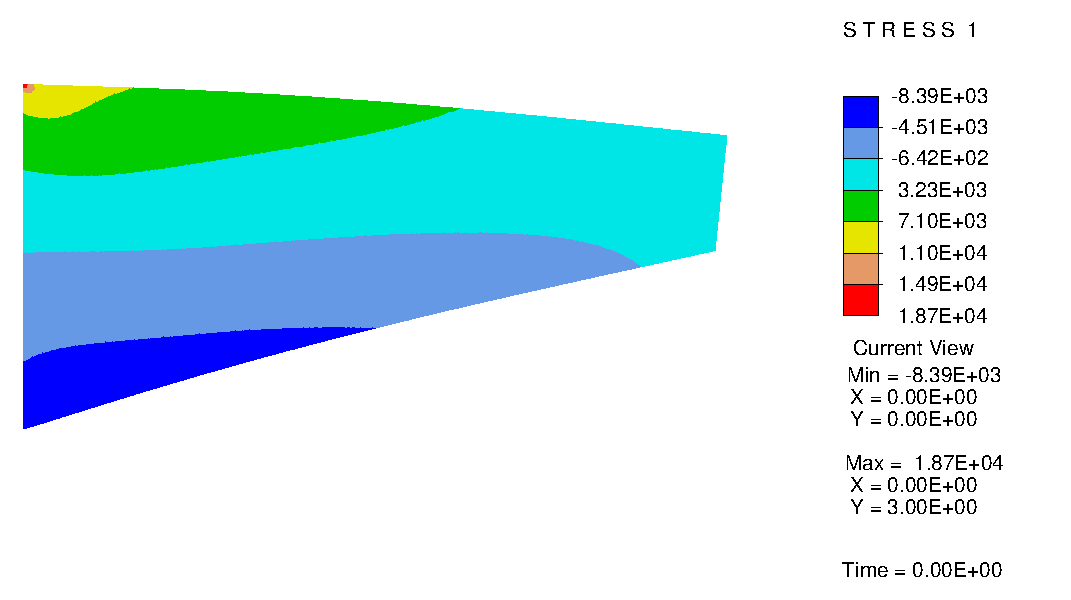
\includegraphics[height=0.32\textheight]{stress11.eps}\\[5mm]
% 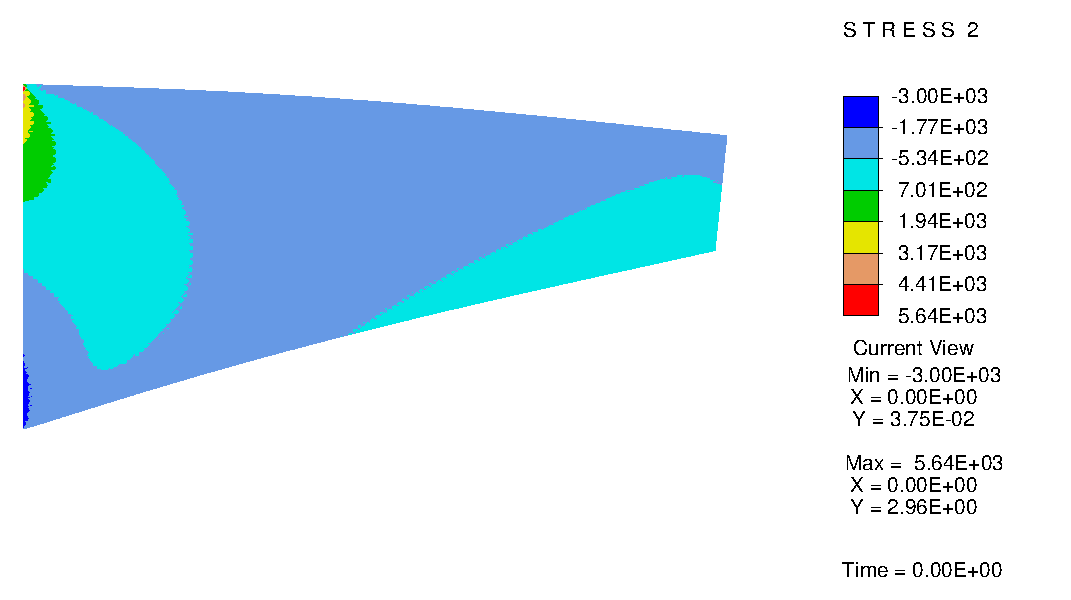
\includegraphics[height=0.32\textheight]{stress22.eps}\\[5mm]
% 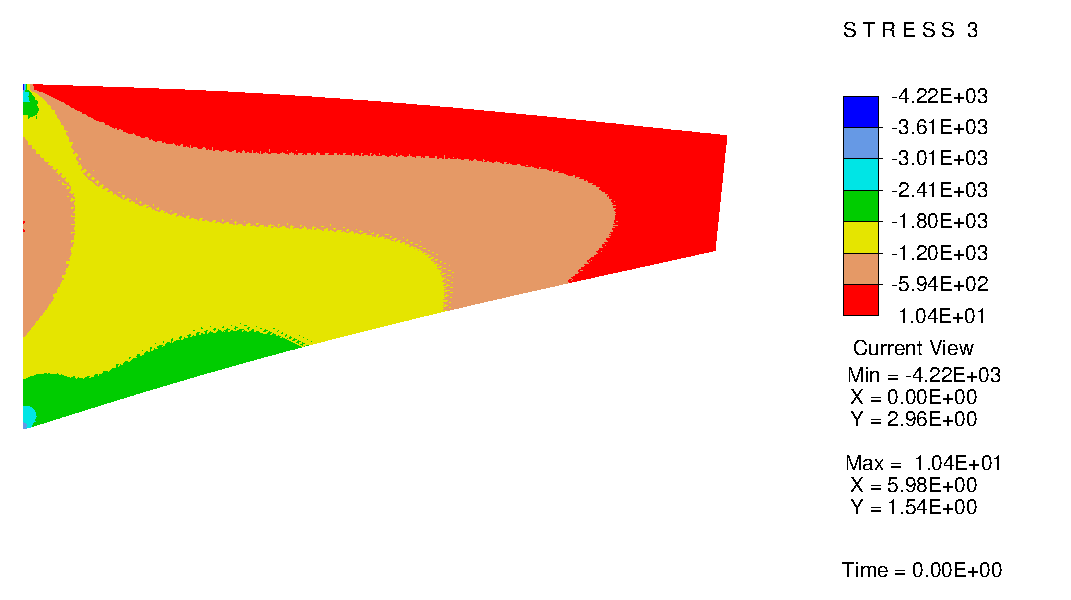
\includegraphics[height=0.32\textheight]{stress33.eps}
% \caption{Stress distributions $\sigma_{11}, \sigma_{22}, \sigma_{33}$}
% \end{figure}

